\documentclass[12pt]{article}
%General Packages
\usepackage{multicol, enumerate, enumitem, hyperref, color, soul, setspace, parskip, fancyhdr}

%Math Packages
\usepackage{amssymb, amsthm, amsmath, bbm, latexsym, units, mathtools}

%All math in Display Style
\everymath{\displaystyle}

% Packages with additional options
%\usepackage[T1]{fontenc}
\usepackage[headsep=0.5cm,headheight=0cm, left=1 in,right= 1 in,top= 1 in,bottom= 1 in]{geometry}
\usepackage[usenames,dvipsnames]{xcolor}

% SageTeX
\usepackage{sagetex}

% Package to use the command below to create lines between items
\usepackage{dashrule}
\newcommand{\litem}[1]{\item#1\hspace*{-1cm}\rule{\textwidth}{0.4pt}}

\pagestyle{fancy}
	\lhead{Module 7 - Rational Functions}
	\chead{}
	\rhead{Progress Exam 3}
	\lfoot{Spring 2019}
	\cfoot{}
	\rfoot{Version C}
	

\begin{document}
	\pagestyle{fancy}

\begin{sagesilent} 
load("../Code/generalPurposeMethods.sage")
load("../Code/keyGeneration.sage")
\end{sagesilent}

\begin{enumerate}
\setcounter{enumi}{30}

\begin{sagesilent}
version = "C"
moduleNumber = 7

problemNumber = 31
load("../Code/rational/domainRational.sage")
\end{sagesilent}

\litem{ \sage{displayStem}
$$ f(x) = \sage{displayProblem} $$
	\begin{enumerate}[label=\Alph*.]
		\item $\sage{choices[0]}$
		\item $\sage{choices[1]}$
		\item $\sage{choices[2]}$
		\item $\sage{choices[3]}$
		\item $\sage{choices[4]}$
	\end{enumerate}		
}

\begin{sagesilent}
problemNumber = problemNumber + 1
load("../Code/rational/solveRationalLinear.sage")
\end{sagesilent}
%TYPE 2 - Exp to Log
\litem{ \sage{displayStem}
	$$ \sage{leftSide} = \frac{\sage{factorNumerator3}}{\sage{factorDenominator3}}  $$
	\begin{enumerate}[label=\Alph*.]
		\item $\sage{choices[0]}$
		\item $\sage{choices[1]}$
		\item $\sage{choices[2]}$
		\item $\sage{choices[3]}$
		\item $\sage{choices[4]}$
	\end{enumerate}	
}

\begin{sagesilent}
problemNumber = problemNumber + 1
load("../Code/rational/solveRationalQuadratic.sage")
\end{sagesilent}

\litem{ \sage{displayStem}
	$$ \sage{firstTerm} - \sage{secondTerm} = \sage{thirdTerm} $$
	\begin{enumerate}[label=\Alph*.]
		\item $\sage{choices[0]}$
		\item $\sage{choices[1]}$
		\item $\sage{choices[2]}$
		\item $\sage{choices[3]}$
		\item $\sage{choices[4]}$
	\end{enumerate}	
}

\newpage 

\begin{sagesilent}
problemNumber = problemNumber + 1
load("../Code/rational/rationalGraphToEquation.sage")
\end{sagesilent}

\litem{ \sage{displayStem}

\begin{multicols}{2}
\begin{center}
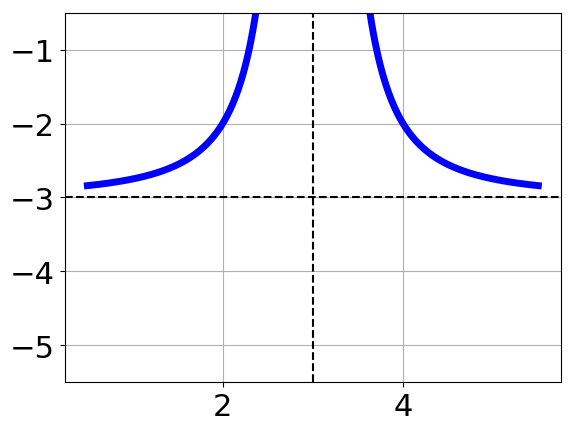
\includegraphics[width=.4\textwidth]{../Figures/question34A.png}
\end{center}

\columnbreak

	\begin{enumerate}[label=\Alph*.]
		\item $f(x) = \sage{choices[0]}$ 
		\item $f(x) = \sage{choices[1]}$ 
		\item $f(x) = \sage{choices[2]}$ 
		\item $f(x) = \sage{choices[3]}$  
	\end{enumerate}
\end{multicols}	
}

\begin{sagesilent}
problemNumber = problemNumber + 1
load("../Code/rational/rationalEquationToGraph.sage")
\end{sagesilent}

\litem{ \sage{displayStem}
$$ f(x) = \sage{displayProblem} $$

	\begin{enumerate}[label=\Alph*.]
\begin{multicols}{2}
		\item \begin{center}
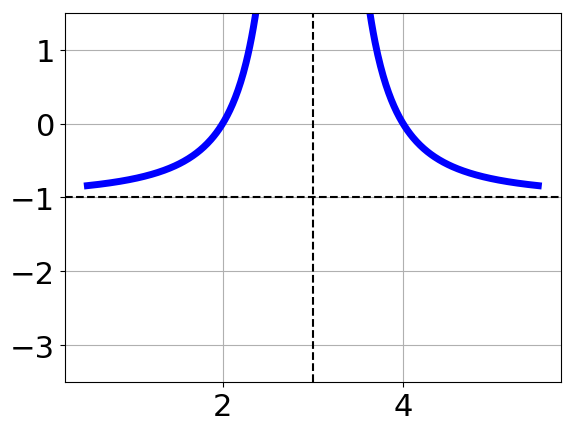
\includegraphics[width=.3\textwidth]{../Figures/question35AA.png}
\end{center}
		\item \begin{center}
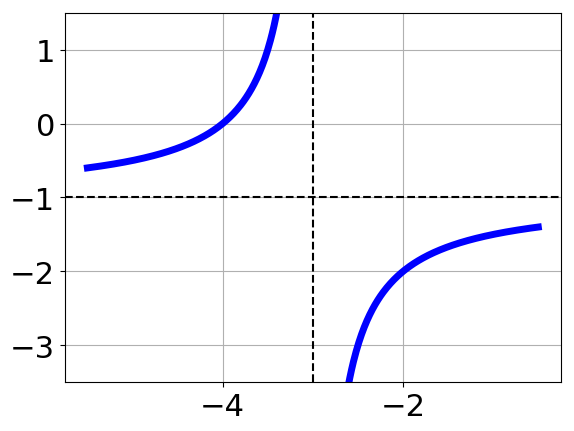
\includegraphics[width=.3\textwidth]{../Figures/question35AB.png}
\end{center}
\columnbreak
		\item \begin{center}
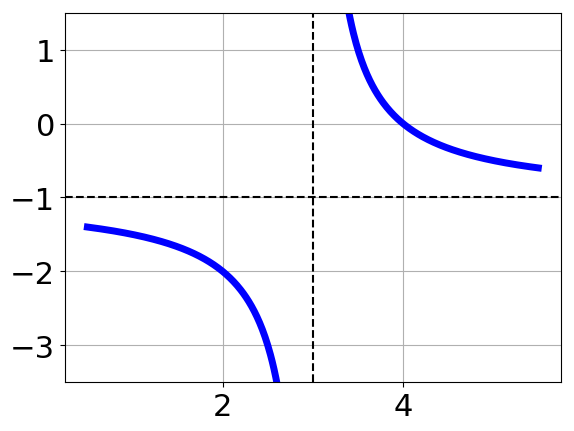
\includegraphics[width=.3\textwidth]{../Figures/question35AC.png}
\end{center}
		\item \begin{center}
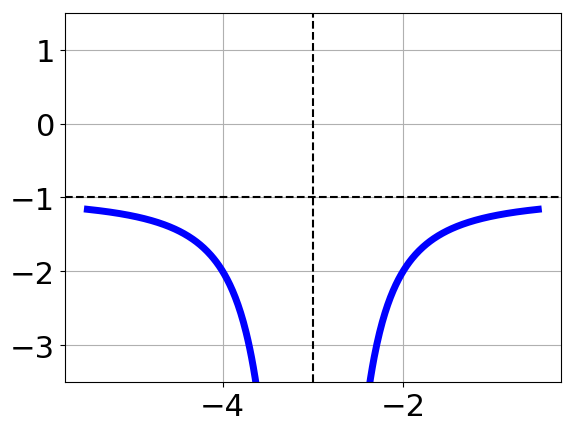
\includegraphics[width=.3\textwidth]{../Figures/question35AD.png}
\end{center}
\end{multicols}
	\end{enumerate}	
}

\end{enumerate}

\end{document}